\scanpage{114}
\margin{\figure{\begin{tikzpicture}\draw (0,0)--(.02,-.8);\end{tikzpicture}}}
est de plus propre, alors pour \uline{toute} sous-variété linéaire $\inserted{L_t}$ de codimensio\handwritten{n} $s$, $Y_t=f_t^{-1}(L_t)$ est géométriquement connexe.

Conjuguant avec 2, on trouve, par l'argument qui a permis de déduire 3 de 1 :

\margin{\handwritten{cf. SGA 1 X \unsure{2.11|2,11|2.II}}}
\margin{\figure{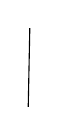
\begin{tikzpicture}\draw (.02,0)--(0,-1);\end{tikzpicture}}}
\uline{Corollaire} 5: \deleted{Avec}\inserted{\handwritten{Sous}} les hypothèses de \unsure{\deleted{4}3|\deleted{3}4}, \inserted{avec $X$ propre,} l'homomorphisme danonique $\handwritten{\pi}_1(Y_{\bar{t}})\handwritten{\rightarrow}\handwritten{\pi}_1(X)$ ($\handwritten{\simeq}\handwritten{\pi}_1(X_{\bar{t}})$ par le théorème de changement de base) est surjectif.

Nous désirons également un énoncé analogue à 5, donnant une surjectivité pour des $\handwritten{\pi}_1$ pour un $t$ non générique, mais sans hypothèse de propreté, et pour des quotients plus gros du $\handwritten{\pi}_1$ que ceux envisagés dans (**). On peut\deleted{\unsure{on|nt}} donner à ce sujet le résultat suivant:

\margin{\figure{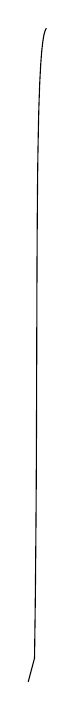
\begin{tikzpicture}\draw (.15,0) .. controls (-.02,-.2) and (.06,-4) .. (0,-8) --(-.08,-8.3);\end{tikzpicture}}}
\uline{Théorème} 6. \unsure{Supposons|Suipposons} $k$ algébriquement clos, \inserted{\handwritten{et}} $X$ propre, $f:X\handwritten{\rightarrow}P^r$, \deleted{et} le sous -espace linéaire $L_t$ de $P^r$ de codimension $s$ (défini sur $k$, pour fixer les idées) \deleted{tels qu'on ait} et enfin le sous-schéma fermé $D$ de $X$ tels qu'on ait ceci; \deleted{où on a posé $U=X-D$}

a) \deleted{$\unsure{U}_t=\unsure{U}\unsure{\cap}X_t$ et} $\deleted{X}\handwritten{Y}_t=f^{-1}(L_t)$ est non vide.

b) Pour tout $x\handwritten{\in}\deleted{X}\handwritten{Y}_t$, $X$ est lisse en $x$, $Y_t$ est lisse en $x$\handwritten{,} de codi\unsure{\deleted{mem}men|\deleted{men}mem}sion $s$ dans $X$ en $x$, $f$ est net en $x$.

c) Pour tout $x\handwritten{\in}D_t=D\handwritten{\cap}Y_t$, o\deleted{\`{}}u \deleted{bien} bien $\operatorname{codim}_x(D_t,\deleted{\unsure{X|T}}\handwritten{Y}_t)\handwritten{\geq}2$, ou bien $D_{\deleted{\unsure{t}}}$ est un diviseur \unsure{enr|sur} $X$ en $x$ et $\deleted{D_t}$ induit sur $Y_t$ en $x$ un diviseur à croisements normaux.

\unsure{Supposons|Suipposons} $U=X-D$ irréductible, et considérons l'inclusion $U_t=U\handwritten{\cap}Y_t\handwritten{\longrightarrow}U$. \deleted{Alors $\unsure{U|Y}_t$} Soit $\handwritten{\pi}_1^t(U)$ le \deleted{\unsure{grou|gros}} quotient du groupe fondamental de $U$ \deleted{formé des} qui classifie les revêtements de $U$ qui sont modérément ramifiés en les composantes irréductibles de codimension 1 de $D$ dans $X$ qui rencontrent $Y_t$, \deleted{(\unsure{i.e.} telles que $D$} et $\handwritten{\pi}_1^t(\unsure{\mathbb{U}|\deleted{V}U|\deleted{U}V|\mathbb{V}}_t)$ le quotient \deleted{analogue} de $\handwritten{\pi}_1(U_t)$ qui classifie les revêtements qui sont modérément ramifiés en les composantes irréductibles de codimension 1 de $D_t$. On a un homomor%
% archive sheet number: 113
